\documentclass[12pt, letterpaper]{article}
\usepackage{graphicx} % Required for inserting images
\usepackage{hyperref}
\usepackage{listings}
\usepackage{amssymb}
\usepackage{amsmath}
\usepackage[english]{babel}
\usepackage{nicefrac, xfrac}
\usepackage{mathtools}
\usepackage[table,xcdraw]{xcolor}
\definecolor{light-gray}{gray}{0.95}
\definecolor{sap}{RGB}{130, 36, 51}
\definecolor{lg}{RGB}{102, 161, 95}
\usepackage[paper=a4paper,left=20mm,right=20mm,bottom=25mm,top=25mm]{geometry}
\newcommand{\code}[1]{\colorbox{light-gray}{\texttt{#1}}}
\newcommand{\codee}[1]{\colorbox{white}{\texttt{#1}}}
\newcommand{\acc}{\\\hphantom{}\\}
\newcommand{\dete}{{\rightarrow}}
\newcommand{\fdot}{{\(\bullet\) }}
\newcommand{\boxedMath}[1]{\begin{tabular}{|c|}\hline \texttt{#1} \\ \hline\end{tabular} :}
\title{Basi di Dati 2}
\author{Marco Casu}
\date{\vspace{-5ex}}
\begin{document}



\maketitle
\begin{figure}[h]
    \centering{
    
\includegraphics[width=1\textwidth ]{images/copertina.jpeg}
    }
\end{figure}
\newpage 
\tableofcontents
\newpage
\section{Introduzione}
Questo corso non è ristretto esclusivamente alla progettazione di basi di dati, bensì fornisce 
cenni sulla progettazione di software di grandi dimensioni, supportati da basi di dati reali.\acc 
Un cliente (committente) fornisce delle specifiche riguardo un progetto che bisogna sviluppare, 
esso stesso non sa come verrà implementato o quali sono nello specifico tutte le funzionalità, 
un insieme di ingegneri del software, progettisti, e programmatori si occuperanno di "tirare su" il 
lavoro completo nel tempo, e varie figure professionali verranno necessariamente coinvolte.\acc 
\textit{Tempi per un progetto software complesso} :\begin{itemize}
    \item Capire il problema e cosa vuole realmente il cliente : \(33\%\) del tempo totale.
    \item Progettazione, capire come implementare le richieste del cliente : \(50\%\) del tempo totale.
    \item Effettiva realizzazione (sviluppo del codice) : \(17\%\) del tempo totale.
    \item Del tempo extra per i test di verifica e la manutenzione.
\end{itemize}
\subsection{Contesto Organizzativo}
Le figure professionali \textit{chiave} coinvolte nel progetto sono dette \textbf{attori}, generalmente
sono :\begin{itemize}
    \item Committente ed Esperti del dominio 
    \item Analisti e Progettisti
    \item Programmatori 
    \item Utenti finali e Manutentori
\end{itemize}
Qual'è la differenza tra analisti e progettisti? E di cosa si occupano gli esperti del dominio?\acc 
Il \textbf{dominio} dell'applicazione è l'insieme di informazioni necessarie da conoscere per poter lavorare 
ad un progetto che fa riferimento ad uno specifico ambito, ad \textit{esempio}, un applicazione che si occupa 
di registrare e gestire le contravvenzioni stradali, vedrà sicuramente nel suo dominio il codice stradale 
e le informazioni legislative. \acc L'esperto del dominio è una figura, appunta esperta, del dominio inerente 
al progetto in questione, viene pagata dal committente e funge da consulente durante lo sviluppo.
\subsection{Ciclo di Vita del Software}
È possibile suddividere lo sviluppo di un software in macro-fasi principali.\begin{enumerate}
    \item \textbf{Studio di fattibilità} - Ci si approccia al progetto valutando i costi per realizzarlo ed 
    i benefici, si pianificano le attività e le risorse del progetto, umane ed economiche, e si individua l'ambiente
    di programmazione hardware e software. 
    \item \textbf{Raccolta dei requisiti} - Bisogna capire \textit{cosa il sistema deve fare}, scrivere in prosa 
    una documentazione che descriva precisamente le usabilità del progetto, sintetizzando i requisiti, che spesso 
    sono contraddittori, trovando i giusti compromessi.
    \item \textbf{Analisi concettuale dei requisiti} - Sono coinvolti gli analisti, che produrranno uno schema 
    matematico del progetto, dettagliato per filo e per segno, che definirò cosa l'applicazione deve fare 
    indipendentemente dal come. Lo schema prima citato è detto \textit{schema concettuale}, e sarà la base 
    da cui partire per la progettazione.
    \item \textbf{Progettazione (design) dell'applicazione} -  Bisogna capire \textit{come} il sistema 
    realizzerà le sue funzioni, entra in gioco il progettista, che definirà l'architettura volta ad ospitare 
    il software e l'insieme delle tecnologie necessarie.
    \item \textbf{Realizzazione} - Una volta che si hanno le linee guida per la realizzazione, composte 
    nelle fasi precedenti, si delega la scrittura del codice ai programmatori, che non sono coinvolti nel resto 
    e non devono necessariamente essere a conoscenza di cosa stanno facendo, ma esclusivamente produrre 
    le funzioni richieste.
    \item \textbf{Verifica, esercizio e manutenzione} - Le diverse componenti dell'applicazione vengono 
    integrate. Una volta che il progetto è realizzato e pronto alla 
    messa in esercizio, si passa da una fase di testing ad una fase di utilizzo effettivo, l'applicazione verrà 
    monitorata durante l'esercizio ed eventuali correzzione verranno prodotte.
\end{enumerate}
Si osservi il seguente diagramma rappresentante il \textbf{modello a spirale} di realizzazione : \begin{center}
    \includegraphics[width=0.65\textwidth ]{images/cicloDiVita.eps}
\end{center}
Tutto il progetto viene costruito in maniera "iterativa", si dice che lo sviluppo del software sia 
\textit{agile}, si comincia raccogliendo i requisiti strettamente necessari, per poi procedere all'analisi 
considerando tali requisiti, con l'andare avanti delle fasi portando alla realizzazione di una prima versione 
del software, pronta ad essere messa in esercizio, implementante esclusivamente le funzionalità di base, tale 
versione renderà chiare le idee al committente che potrà fornire nuovi requisiti, in modo tale da ricominciare il ciclo.\acc 
Nulla vieta alle varie fasi di essere eseguite in parallelo, ad esempio, nel tempo \(t_0\) vengono stilati 
i requisiti per la prima versione del software, nel tempo \(t_1\) gli analisti iniziano a produrre il modello della versione 1, ma 
possono essere nel mentre stilati i requisiti della versione 2, al tempo \(t_3\), com'è di facile intuzione : 
 Si raccolgono i requisiti per la versione 3, si produce il modello della versione 2, si progetta la versione 1.
 \subsection{Il linguaggio UML}
Il linguaggio UML, acronimo di \textit{Unified Modeling Language}, nasce con l'intento di definire un 
linguaggio logico-matematico e formale per la progettazione del software. Utilizza dei diagrammi con lo scopo di 
"sintetizzare" un linguaggio puramente logico. \acc 
Verrà utilizzato l'UML per modellare il dominio applicativo ed i dati di interesse, utilizzeremo il cosiddetto 
\textbf{diagramma delle classi e degli oggetti}. Un \textit{oggetto} modella un elemento del dominio di business, 
la cui esistenza è "autonoma", e può essere identificato appunto come un "oggetto" del mondo reale, identifica una classe, 
di cui è "estensione", in maniera similare ai linguaggi object-oriented\acc Sarà importante concentrarsi sulle classi 
piuttosto che sugli oggetti specifici, una classe definisce un nome identificativo, degli attributi e delle 
operazioni.\begin{center}
    \includegraphics[width=\textwidth ]{images/umlBase.eps}
\end{center}
Una classe permette di modellare oggetti dello specifico tipo definito da essa, un oggetto ha un identificatore 
univoco (sottolineato), possono però esistere due oggetti identici, a patto che differiscano per 
l'identificatore.
\subsection{Associazioni e Link}
Un \textit{associazione} definisce un legame fra due oggetti istanza di due classi diverse, si denota con una freccia o linea che collega due classi, 
e deve presentare un titolo, ad esempio, un oggetto di tipo \textit{Libro}, può essere associato ad un oggetto 
di tipo \textit{Persona} tramite un'ipotetica associazione \textit{autore}.\begin{center}
    \includegraphics[width=\textwidth ]{images/associazione.eps}
\end{center}
Un \textit{link} non è altro che il corrispettivo delle associazioni, ma sugli oggetti istanza delle classi. Due oggetti 
identici possono esistere, ma due link identici fra due oggetti no, si immagini l'esempio precedente di autore, 
non avrebbe senso che una persona sia due volte autore dello stesso libro.\begin{center}
    \includegraphics[width=0.8\textwidth ]{images/2link.eps}
\end{center}
\subsubsection{Classi Ponte e Molteplicità}
Si consideri adesso il seguente esempio, si vuole progettare un'applicazione che gestire le prenotazioni di un 
hotel, e si produce il seguente modello UML, con le classi \textit{Hotel} e \textit{Persona} unite dall'associazione 
"prenota", cosa succederebbe se una persona volesse prenotare 2 volte lo stesso hotel? \begin{center}
    \includegraphics[width=0.7\textwidth ]{images/hotelSbagliato.eps}
\end{center}
Non è giusto modellare la prenotazione come un associazione, in quanto vogliamo che le prenotazioni esistano come 
oggetti autonomi, e che uno stesso cliente possa prenotare più volte lo stesso hotel, si necessita di una classe 
prenotazione che si occupi di tale relazione, una classe di questo tipo è detta \textbf{classe ponte}, e nel 
caso degli hotel, viene 
implementata nel seguente modo : \begin{center}
    \includegraphics[width=0.9\textwidth ]{images/hotelGiusto.eps}
\end{center}
Ovviamente, fra le stesse due classi, possono esistere più associazioni diverse, ad esempio, le classi 
\textit{Libro} e \textit{Persona}, potrebbero essere relazionate da \textit{autore} ed \textit{editore}. Inoltre, 
un oggetto di una classe \(C_1\), può essere collegato tramite link a due oggetti diversi di una stessa classe 
\(C_2\), ciò è valido, ma potrebbe causare alcuni errori logici : \begin{center}
    \includegraphics[width=1\textwidth ]{images/multError.eps}
\end{center}
Nonostante lo schema relazionale permetta tali istanze, il fatto che una persona sia nata in due città differenti 
non rispetta i vincoli del mondo reale, il diagramma è quindi troppo \textit{lasco}, appositamente per situazioni 
di questo tipo, esistono dei costrutti, detti \textbf{vincoli di molteplicità} sulle associazioni, che restringono 
il possibile numero delle istanze, imponendo delle restrizioni sul numero di link che possono esistere fra due classi.
\begin{center}
    \includegraphics[width=1\textwidth ]{images/molteplicita.eps}
\end{center} 
I vincoli di molteplicità vengono aggiunti ai terminali della linea associazione : \begin{itemize}
    \item il vincolo \textbf{0..*} posto al terminale della classe \textit{A}, in associazione con la 
    classe \textit{B} implica che ogni istanza della classe \textit{A}, dovrà essere coinvolta in un numero di link 
    dell'associazione in questione, che va da 0 ad un qualsiasi numero (ogni istanza di \textit{A} può essere legata 
    ad un numero qualunque di istanze di \textit{B}).
    \item il vincolo \textbf{1..1} posto al terminale della classe \textit{A}, in associazione con la 
    classe \textit{B} implica che ogni istanza della classe \textit{A}, dovrà essere coinvolta in un numero di link 
    dell'associazione in questione, che va da 1 ad 1 (ogni istanza di \textit{A} sarà collegata ad una sola 
    istanza di \textit{B}).
    \item (caso generale) il vincolo \textbf{\(k\)..\(n\)} posto al terminale della classe \textit{A}, in associazione con la 
    classe \textit{B} implica che ogni istanza della classe \textit{A}, dovrà essere coinvolta in un numero di link 
    dell'associazione in questione, che va da \(k\) ad \(n\).
\end{itemize}\begin{center}
    \includegraphics[width=\textwidth ]{images/esempioAuto.eps}
\end{center}
Si considerino i seguenti requisiti : Si vogliono rappresentare i sovrani 
di un regno, di ognuno di loro, è importante considerare il predecessore 
ed il successore, è possibile in UML creare un link fra due oggetti della 
stessa classe, con un associazione sulla stessa classe : \begin{center}
    \includegraphics[width=0.5\textwidth ]{images/sovrani.eps}
\end{center}
Risulta però \textit{obbligatorio} dare dei nominativi ai \textbf{ruoli}
posti ai terminali dell'associazione, altrimenti sarebbe impossibile quale 
delle due classi sta interpretando il ruolo di successore o predecessore. 
Vorremmo inoltre che ogni sovrano, eccetto il primo e l'ultimo, abbia esattamente 
un successore ed un predecessore, ma il diagramma in questione permette a qualunque 
sovrano di violare tali vincoli del mondo reale.
\subsubsection{Associazioni con Attributi}
Si vuole progettare un sistema che gestisca gli esiti (voti in 30esimi) di 
più esami sostenuti dagli studenti di un corso di laurea, esisteranno sicuramente 
le classi \textit{Studente} ed \textit{Esame}.\acc 
Il problema, è che non è possibile utilizzare una classe ponte, in quanto 
deve essere impossibile per uno studente, superare lo stesso esame più di una volta. Sarebbe 
naturale inserire il voto dell'esame in questa ipotetica classe ponte, ma sapendo che non 
è utilizzabile, dove verrà inserito l'attributo \textit{voto}?
\begin{center}
\includegraphics[width=0.8\textwidth ]{images/votoSbagliato.eps}
\end{center}
 Chiaramente, non posso inserirlo nella classe \textit{Studente}, in quanto 
 ogni studente avrebbe un unico voto per ogni esame, e non posso inserirlo 
 nella classe \textit{Esame}, dato che tutti gli studenti avrebbero lo 
 stesso voto nello stesso esame. \acc 
 È possibile considerare degli \textbf{attributi di associazione}, dando 
 ad ogni link di \textit{testSuperato}, il corrispettivo valore del voto, risulta 
 una soluzione naturale, in quanto il voto è assegnato ad ogni superamento di un test :\begin{center}
    \includegraphics[width=0.8\textwidth ]{images/votoGiusto.eps}
    \end{center} 
Anche se simile, il riquadro \textit{votoSuperato} non rappresenta una 
classe, in UML è detta \textit{association class}, e anche essa può essere collegata ad 
altre classi, si supponga ad esempio che vogliamo associare ad ogni 
test superato, anche il docente che ha verbalizzato il voto, basta 
collegare l'associazione con attributi ad una classe \textit{Docente} : \begin{center}
    \includegraphics[width=0.8\textwidth ]{images/conDocente.eps}
    \end{center} 
\subsection{Tipi di Dato} 
Per ogni attributo di ogni classe abbiamo visto essere necessario 
considerare il tipo del dato, esiste infatti un insieme di tipi di 
dato \textit{concettuali}, che siano facilmente implementabili 
in modo ovvio su qualsiasi sistema o linguaggio di programmazione.\begin{center}
    \code{Intero, Reale, Booleano, Data, Ora, DataOra}
\end{center}
\end{document}
